\documentclass[a4paper, 12pt]{article}
\usepackage{amsmath}
\usepackage{graphicx}
\usepackage{caption}
\usepackage{float}
\usepackage{minted}
\usepackage{xcolor}
\definecolor{LightGray}{gray}{0.9}
\usepackage{ragged2e}

\title{STK1100 - Obligatorisk oppgavesett 1 av 2}
\author{Klaudia M. Pawlak}
\date{17.02.2020}
\begin{document}
\maketitle

\section*{Oppgave 1}

\subsection*{a)}
Sannsynligheten for at de 5 personene går av i hver sin etasje er:
\[
P(\text{hver etasje}) = \frac{11 \cdot 10 \cdot 9 \cdot 8 \cdot 7}{11^5} = \frac{5040}{161051} \approx 0.344
\]

\subsection*{b)}
Sannsynligheten for at minst 2 av de 5 går av i samme etasje er:
\[
P(\text{minst 2 går av i samme etasje}) = 1 - P(\text{hver etasje}) = 1 - 0.344 = 0.656
\]

\subsection*{c)}
Vi velger 3 personer fra en gruppe på 5:
\[
\binom{5}{3} = \frac{5 \cdot 4}{2} = 10
\]
Sannsynligheten for at nøyaktig tre personer går ut på 8. etasje er:
\[
\binom{1}{11}^3 \cdot \binom{10}{11}^2 = \frac{100}{161051} \approx 0.00062
\]
Vi får:
\[
10 \cdot 0.00062 = 0.0062
\]

\subsection*{d)}
Sannsynlighet for at delene (1,2) virker:
\[
1 - 0.1 \cdot 0.1 = 0.99
\]
Sannsynlighet for at (3,4,5) virker:
\[
0.99 \cdot 0.9 = 0.891
\]
Så sannsynligheten for at alarmen i heisen virker er:
\[
1 - 0.01 \cdot 0.109 = 0.99891
\]

\section*{Oppgave 2}

\begin{itemize}
    \item \( P(M) \) = Sannsynlighet for at Martin mater fisken
    \item \( P(\neg M) \) = Sannsynlighet for at Martin glemmer å mate fisken
    \item \( P(O \mid M) \) = Sannsynlighet for at fisken overlever ferien dersom Martin mater den
    \item \( P(O \mid \neg M) \) = Sannsynlighet for at fisken overlever ferien dersom Martin ikke mater den
\end{itemize}

\begin{FlushLeft}
Vi har gitt at sannsynligheten for at Martin glemmer å mate fisken er \( \frac{1}{4} \). Altså: 
\end{FlushLeft}
\[
P(\neg M) = \frac{1}{4}
\]
\begin{FlushLeft}
Derfor blir sannsynligheten for at Martin mater fisken:
\end{FlushLeft}
\[
\quad P(M) = 1 - \frac{1}{4} = \frac{3}{4}
\]
\begin{FlushLeft}
Sannsynlighet for at fisken overlever ferien dersom Martin mater den er:
\end{FlushLeft}
\[
P(O|M) = \frac{9}{10}
\]
\begin{FlushLeft}
Sannsynlighet for at fisken overlever ferien dersom Martin ikke mater den er:
\end{FlushLeft}
\[
\quad P(O|\neg M) = \frac{1}{2}
\]
\begin{FlushLeft}
Sannsynlighet for at fisken overlever ferien:
\end{FlushLeft}
\[
P(O) = P(O|M) \cdot P(M) + P(O|\neg M) \cdot P(\neg M)
\]
\[
= \frac{9}{10} \cdot \frac{3}{4} + \frac{1}{2} \cdot \frac{1}{4} = \frac{32}{40} = \frac{4}{5}
\]
\begin{FlushLeft}
Så sannsynligheten for at fisken ikke overlever ferien er:
\end{FlushLeft}
\[
P(\neg O) = 1 - \frac{4}{5} = \frac{1}{5}
\]
\begin{FlushLeft}
Vi bruker Bayes-setningen:
\end{FlushLeft}
\[
P(\neg M|\neg O) = \frac{P(\neg O|\neg M) \cdot P(\neg M)}{P(\neg O)}
\]
\[
= \frac{\frac{1}{2} \cdot \frac{1}{4}}{\frac{1}{5}} = \frac{5}{8}
\]
\begin{FlushLeft}
Sannsynligheten for at Martin har glemt å mate fisken og derfor den døde er:
\end{FlushLeft}
\[
\frac{5}{8}
\]

\section*{Oppgave 3}
\subsection*{a)}
Vi har at:
\begin{itemize}
    \item \(X\) = Mannens gjenstående levetid i hele år
    \item \(q_x\) = Sannsynligheten for at en \(x\) år gammel mann skal dø i løpet av ett år
\end{itemize}

\begin{FlushLeft}
Mannen er 35 år gammel nå. Av produktsetningen har vi:
\end{FlushLeft}
\[
P(X > x) = P(X > 0) \cdot P(X > 1|X > 0) ... P(X > x|X > x-1)
\]
\[
= (1 - q_{35})\cdot(1 - q_{36})...(1 - q_{x})
\]
\begin{FlushLeft}
Den kumulative fordelingsfunksjonen blir derfor:
\end{FlushLeft}
\[
F(x) = P(X \leq x) = 1 - P(X > x)
\]
\[
F(x) = 1 - \prod_{y=0}^{x} (1 - q_{35+y})
\]

\subsection*{b)}
Punktsannsynligheten er gitt som:
\[
p(x) = P(X = x)
\]
For to ulike verdier \(a\) og \(b\), hvor \(a\leq b\) , vil punktsannsynligheten bli gitt som:
\[
P(a\leq X \leq b) = F(b)-F(a-)
\]
For å finne ut sannsynligheten for mannens eksakte gjenstående levetid, trenger vi to andre sannsynligheter. En sannsynlighet for at mannen dør i løpet av \(x\) år, og en sannsynsynlighet for at mannen dør i løpet av \(x-1\) år. Altså:
\[
p(x) = P(X = x) = F(x) - F(x-1)
\]
Vi regner 106 år som den høyest mulige levealder. Mannen er 35 år gammel nå, så mannens gjenstående levetid er 71 år.
For 
\[
x = 0,1,2, . . . ,71 \text{ hvor x er et positivt heltall} 
\]
Har vi at:
\[
p(x)=F(x)-F(x-1)
\]

\subsection*{c)}

Python-kode:
\begin{minted}
[
bgcolor=LightGray,
fontsize=\footnotesize,
linenos
]
{python}
import numpy as np
import matplotlib.pyplot as plt
import pandas as pd

url = "https://www.uio.no/studier/emner/matnat/math/STK1100/v20/doedelighet.txt"
doed = pd.read_csv(url, sep="\t")
alder = doed["alder"].values
menn = doed["menn"].values

qx = menn[35:]/1000
Sx = np.cumprod(1-qx)
Fx = 1-Sx

tmp = np.zeros(72)
tmp[1:72] = Fx[0:71]
px = Fx - tmp

x = alder[35:]

plt.bar(x, px, width=1, edgecolor="black")
plt.xlabel("Alder")
plt.ylabel("Punktsannsynlighet")
plt.show()
\end{minted}
\begin{FlushLeft}
Kjøreeksempel gir:
\end{FlushLeft}

\begin{figure}[h]
    \centering
    
\includegraphics[width=0.5\linewidth]{figure1.jpg}
    \caption{Plott av punktsannsynligheten}
    \label{fig:enter-label}
\end{figure}

\subsection*{d)}
\begin{FlushLeft}
Variabelen \(X\) angir mannens gjenstående levetid i hele år, dvs. levetiden i hele år fratrukket 35 år. Det betyr at for \(X \leq 31\) vil mannen dø før han fyller 67 år, og
dermed vil han ikke motta noen pensjonsutbetalinger. Derfor blir \(h(X)=0\).
\end{FlushLeft}
\begin{FlushLeft}
Forsikringsselskapet benytter en rentefot på \(3\%\) pro anno. Nåverdien av \(B\) kroner som betales om \(k\) år er lik \(\frac{B}{{1.03}^{k}}\). Hvis han blir minst 67 år, får han utbetalt \(100000\) kr hvert år, da blir \(B\) verdien lik \(100000\). Og vi får:
\end{FlushLeft}
\[
h(X) = \sum_{k=32}^{X} \frac{100000}{{1.03}^{k}}
\]
\begin{FlushLeft}
Dette er summen av en endelig geometrisk rekke:
\end{FlushLeft}
\[
\sum_{k=0}^{X} a^{k} = \frac{1-{a}^{n+1}}{1-a}
\]
Vi setter \(n=X-32\), og \(a= \frac{1}{1.03}\)
. Så for \(X \geq 32\) blir nåverdien av mannens samlede
pensjonsutbetalinger lik:
\[
h(X) = \frac{100000}{{1.03}^{32}} \sum_{k=0}^{X-32} (\frac{1}{1.03})^{k} = \frac{100000}{{1.03}^{32}} \cdot \frac{1-({\frac{1}{1.03})}^{X-31}}{1-{\frac{1}{1.03}}}
\]

\subsection*{e)}
\begin{FlushLeft}
For å finne forventet nåverdi av pensjonsutbetalingene trenger vi punktsannsynligheten \( p(x) \) og funksjonen \( h(X) \) av \( X \). Ved å addere produktet av disse to, vil vi til slutt få en forventningsverdi \( E[h(x)] \), altså:
\end{FlushLeft}
\[
E[h(x)] = \sum_{x=0}^{71} h(x)p(x)
\]
\begin{FlushLeft}
Vi gjentar forsøket 71 ganger siden vi regner 106 år som den høyest mulige levealder, og siden han er 35 år gammal nå, så mannens gjenstående levetid er 71 år.
\end{FlushLeft}
\begin{FlushLeft}
Vi bruker formler for \( h(x) \) og \( p(x) \) fra forrige deloppgaver, og får:
\end{FlushLeft}

\[
E[h(x)] = \sum_{x=0}^{71} h(x) p(x) = \frac{100000}{1.03^{32}} \sum_{x=0}^{71} 
(\frac{1 - \left( \frac{1}{1.03} \right)^{x-31}}{1 - \frac{1}{1.03}}) p(x)
\]

\[
= \frac{100000}{1.03^{32}} \cdot \frac{1}{1 - \frac{1}{1.03}} \sum_{x=0}^{71} \left( 1 - \left( \frac{1}{1.03} \right)^{x-31} \right) p(x)
\]

\[
= \sum_{x=0}^{71} \frac{103^{x-31} - 100^{x-31}}{3 \cdot 103^x} 10^{69} p(x)
\]
\begin{FlushLeft}
Altså:
\end{FlushLeft}
\[
E[h(x)] = \sum_{x=32}^{71} \frac{103^{x-31} - 100^{x-31}}{3 \cdot 103^x} 10^{69} p(x)
\]
\begin{FlushLeft}
Siden for \( X \leq 32 \) blir \( h(X) = 0 \), skriver vi:
\end{FlushLeft}
\[
E[h(x)] = \sum_{x=32}^{71} \frac{103^{x-31} - 100^{x-31}}{3 \cdot 103^x} 10^{69} p(x)
\]
\begin{FlushLeft}
Vi bruker Python (vi fortsetter på programmet fra oppgave 3c), og får:
\end{FlushLeft}

\begin{minted}
[
bgcolor=LightGray,
fontsize=\footnotesize,
linenos
]
{python}
x = np.arange(0, 72)

hx = np.zeros(72)
for i in range(32, 72):
     hx[i] = 100000 * np.sum(1/(1.03 ** np.arange(32, i+1)))

EhX = sum(hx * px)
print("E[h(x)]=", EhX)
\end{minted}
\begin{FlushLeft}
Kjøreeksempel gir:
\end{FlushLeft}
\begin{figure}[h]
    \centering
    
\includegraphics[width=0.5\linewidth]{figure2.jpg}
\end{figure}

\subsection*{f)}
Mannen betaler premie på en konstant verdi \( K \) kr per år. Vi summerer opp 
nåverdiene av alle premieinnbetalingene, med tanke på at forsikringsselskapet 
benytter en rentefot på 3\% per år, og får:

\[
K \cdot g(x) = K \sum_{k=0}^{\text{min}(X,31)} \frac{1}{1.03^k} = \sum_{k=0}^{\text{min}(X,31)} \frac{K}{1.03^k}
\]
\begin{FlushLeft}
Vi setter \(\text{min}(X, 31)\) i grensen, siden mannen ikke skal betale noe etter han fyller 66 år.
Vi ser at \( g(x) \) er summen av en geometrisk rekke:
\end{FlushLeft}
\[
\sum_{k=0}^{x} a^k = \frac{1 - a^{n+1}}{1 - a}
\]
\begin{FlushLeft}
Vi bruker dette og får:
\end{FlushLeft}
\[
g(x) = \sum_{k=0}^{\text{min}(X,31)} \frac{1}{1.03^k} = \frac{1 - \left(\frac{1}{1.03}\right)^{\text{min}(X,31)+1}}{1 - \frac{1}{1.03}}
\]


\subsection*{g)}
For å finne forventet nåverdi av premieinnbetalingene trenger vi punktsannsynligheten \( p(x) \) og funksjonen \( g(X) \) av \( X \). Ved å addere produktet av 
disse to, vil vi til slutt få en forventningsverdi \( E[g(x)] \), altså:
\[
E[h(x)] = \sum_{x=0}^{71} g(x) p(x)
\]
\begin{FlushLeft}
Vi gjentar forsøket 71 ganger siden vi regner 106 år som den høyest mulige levealder, 
og siden han er 35 år gammal nå, så mannens gjenstående levetid er 71 år. Vi bruker formelen for \( g(x) \), og får:
\end{FlushLeft}
\[
E[h(x)] = \sum_{x=0}^{71} (\frac{1 - \left(\frac{1}{1.03}\right)^{\text{min}(X,31)+1}}{1 - \frac{1}{1.03}})p(x)
\]
\begin{FlushLeft}
Vi bruker Python (vi fortsetter på programmet fra oppgave 3e) og får:
\end{FlushLeft}

\begin{minted}
[
bgcolor=LightGray,
fontsize=\footnotesize,
linenos
]
{python}
gx = (1 - (1/1.03)**(np.minimum(x,31)+1))/(1 - (1/1.03)) 
EgX = sum(gx*px) 
print("E[g(x)]=", EgX)
\end{minted}
\begin{FlushLeft}
Kjøreeksempel gir:
\end{FlushLeft}
\begin{figure}[h]
    \centering
    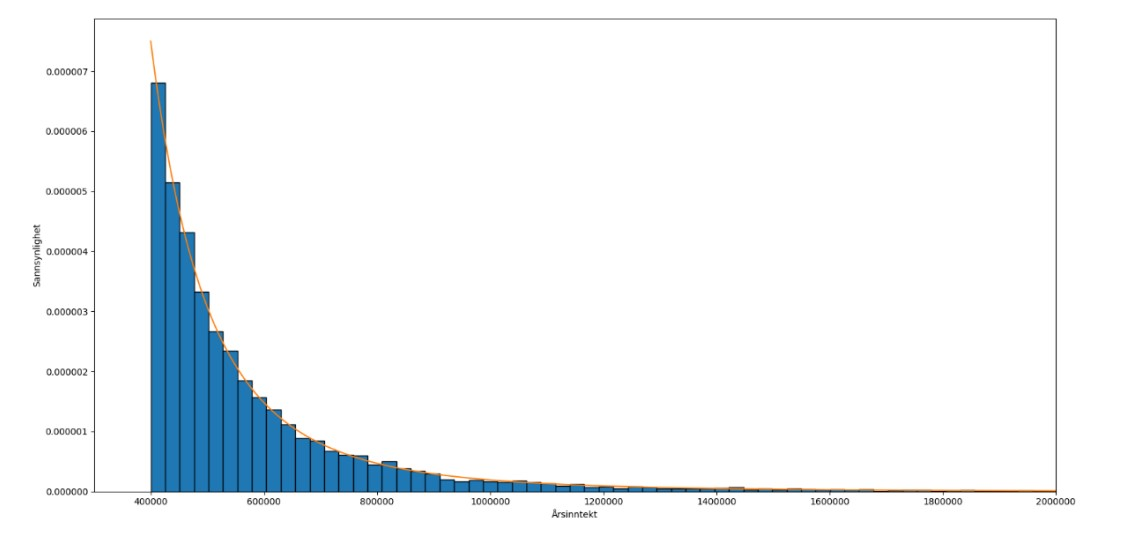
\includegraphics[width=0.5\linewidth]{figure3.jpg}
\end{figure}

\subsection*{h)}
Premien \( K \) bestemmes ved:
\[
K \cdot {E[g(X)]}={E[h(X)]}
\]
\[
K = \frac{E[h(X)]}{E[g(X)]} = 22822.09
\]
\end{document}
